\documentclass[12pt]{article}

\setlength{\parindent}{0pt}
\setlength{\parskip}{2mm}

\usepackage{geometry}
 \geometry{
 letterpaper, left=20mm, right=20mm,  top=20mm,
 }
\usepackage{graphicx}
\graphicspath{ {graphics/} }
\usepackage{amssymb}

%%%%%%%%%%%%%%%%%%%%%%%%%%%%%%%%%%%%%%%%%%%%%%%%%
\title{RFC 1: Collisions in Delay-Based ID Encoding Protocol}
%%%%%%%%%%%%%%%%%%%%%%%%%%%%%%%%%%%%%%%%%%%%%%%%%

\author{
	Margot Maxwell \and
	Lizzy Schoen \and
	Noah Strong \and
	Chloe Yugawa
}

\begin{document}

\maketitle

\tableofcontents{}

%%%%%%%%%%%%%%%%%%%%%%%%%%%%%%%%%%%%%%%%%%%%%%%%%

\section{Introduction}

The protocol proposed for this project encodes an unique identification number
in the transmitted signal by the delay between two consecutive pings.
While this method is easy to implement in hardware, and works well in the case
of only a signal transmitter, the addition of multiple transmitters within range
of a receiver brings about the potential for collisions between different
signals.
In some cases, the collisions may be undetectable, leading to incorrect
reporting of nearby crab IDs.
Completely solving this problem will require a change to the underlying
protocol.
However, the likelihood of such collisions may be low enough that we move
forward with this known flaw in the protocol.

\section{Original Protocol}

In the current iteration of our detection and identification protocol, every
transmitter will transmit at the exact same frequency, likely somewhere around
40kHz. This is ideal from a hardware perspective, as the piezoelectric
equipment can be tuned to work on a single frequency with a high degree of
accuracy.

Every transmitter will periodically send out two quick "pings," each separated
by some delay $d$. The value of $d$ will encode the ID of the transmitter.
For example, $d=42$ms may correspond to ID 30, and a delay of $50.5$ms may
correspond to an ID of 38.
Note that these numbers are only examples.
Because the receiving hardware can easily detect the two pings, it can measure
the value of $d$ by calculating the time difference between the rising edges
of the consecutive signals. See Figure 1 for an illustration.

\begin{figure}[h]
\centering
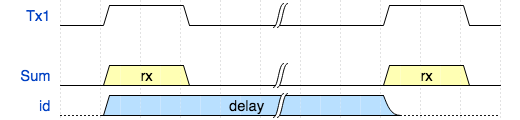
\includegraphics[scale=0.7]{singleTx}

\caption{A single transmitter ($Tx1$), the input received by the receiver
($Sum$), and the calculated delay $d$ based on the time measured between
the rising edges of the two pings from $Tx1$.}
\end{figure}

While this method may be reliable with just a single receiver, it does not work
so well when multiple transmitters are brought into play.

\section{Problem}

\subsection{Details}

\end{document}

